\documentclass[12pt,a4paper,titlepage]{scrartcl}

\usepackage{comment}
\usepackage[main=ngerman,english]{babel}
\usepackage[utf8]{inputenc}
\usepackage[T1]{fontenc}
\usepackage{lmodern}
\usepackage{geometry}
\geometry{left=2.5cm,right=2.5cm,top=2.5cm,bottom=3cm,head=29pt,foot=25pt}
\setlength{\footheight}{25pt}
\usepackage{microtype}
\usepackage{amsmath,amssymb,mathtools}
\numberwithin{equation}{section}
\numberwithin{table}{section}
\numberwithin{figure}{section}
\usepackage{siunitx}
\sisetup{locale=US, separate-uncertainty=true, per-mode=fraction}
\usepackage{booktabs}
\usepackage{multirow}
\usepackage{graphicx}
\usepackage{float}
\usepackage{caption}
\usepackage{subcaption}
\usepackage[automark]{scrlayer-scrpage}
\usepackage[most]{tcolorbox}
\usepackage{hyperref}
\usepackage{pdfpages}
\usepackage{csvsimple-l3}
\usepackage{longtable}
\usepackage{graphicx}

%\input{../../jupyterpackages.tex}

% jupyter nbconvert --to latex 'Path'
% enferne usepackages und begin{document} und end{document}
% \input in main.tex mit \input{Path}


\newcommand{\pdfabbildung}[2]{%
    \refstepcounter{figure}%
    \addcontentsline{lof}{figure}{\protect\numberline{\thefigure}#1}%
    \label{#2}%
}

\newcommand{\pdftabelle}[2]{%
    \refstepcounter{table}%
    \addcontentsline{lot}{table}{\protect\numberline{\thetable}#1}%
    \label{#2}%
}


\hypersetup{colorlinks=true, linkcolor=blue!60!black, urlcolor=blue!60!black, citecolor=blue!60!black}

\clearpairofpagestyles

\chead{%
    \versuch\hfill\autor\\
    \rule{\textwidth}{0.2pt}%
}
\cfoot{%
    \rule{\textwidth}{0.2pt}\\[-0.5ex]
    \pagemark\ 
}
\addtokomafont{pagefoot}{\small}
\setlength{\parindent}{0pt}

\newtcolorbox{resultbox}[1][]{ 
    enhanced,
    colback=black!4!white,
    colframe=black!65!black,
    boxrule=0.8pt,
    arc=0.0mm,
    title=#1,
    fonttitle=\bfseries,
    %drop shadow
}


\newcommand{\versuch}{Versuch 35}
\newcommand{\titel}{Fotoeffekt}
\newcommand{\praktikum}{Physikalisches Anfängerpraktikum 1}
\newcommand{\autor}{Jonathan Gießen}
\newcommand{\gruppe}{Gruppe 8}
\newcommand{\datum}{15. September 2026}
\newcommand{\betreuer}{Jannis Wessel}

\begin{document}

\pagestyle{scrheadings}

\begin{titlepage}



    \centering
    \vspace*{4cm}
    {\large Universität Heidelberg\par}
    {\small Fakultät für Physik und Astronomie\par}
    {\Large \praktikum\par}
    \vspace{0.8cm}
    {\LARGE \bfseries \versuch\ -- \titel\par}
    \vspace{1.5cm}

    \begin{tabular}{ll}
        \textbf{Autor:} & \autor\\
        \textbf{Gruppe:} & \gruppe\\
        \textbf{Betreuer:} & \betreuer\\
        \textbf{Versuchsdatum:} & \datum\\
    \end{tabular}

    \vfill
    \hrulefill\
\end{titlepage}

\tableofcontents

\bigskip
\begin{tcolorbox}[colback=gray!5,colframe=gray!60,boxrule=0.8pt,arc=0.01mm,title=KI-Hinweis]
    Für die sprachliche Formulierung dieses Protokolls wurde in der Einleitung \ref{sec:Einleitung} KI-gestützte Textgenerierung verwendet. Die Tabellen in der Auswertung \ref{sec:Berechnungen der Zahlenwerte} wurden von KI berechnet.
\end{tcolorbox}

\clearpage


\section{Einleitung}\label{sec:Einleitung}
Der fotoelektrische Effekt, dessen theoretische Deutung maßgeblich zur Entwicklung der Quantenmechanik beitrug, demonstriert eindrucksvoll die Existenz von Lichtquanten. Bei der Bestrahlung einer Metalloberfläche mit Licht zeigt sich experimentell, dass die Emission von Fotoelektronen erst ab einer materialabhängigen Mindestfrequenz auftritt. Zudem hängt die kinetische Energie der austretenden Elektronen ausschließlich von der Frequenz des einfallenden Lichts ab, nicht jedoch von dessen Intensität, was im direkten Widerspruch zur klassischen Elektrodynamik steht. Dieses Phänomen lässt sich durch die Quantisierung der elektromagnetischen Strahlung in Photonen der Energie $E = h\nu$ erklären, die beim Auftreffen ihre gesamte Energie an die Leitungselektronen des Metalls abgeben.  

In diesem Versuch wird die Emission von Elektronen aus einer Fotokathode experimentell nachgewiesen und untersucht. Das Hauptziel des Versuchs besteht darin, die maximale kinetische Energie der emittierten Fotoelektronen als Funktion der Lichtfrequenz zu messen. Hierzu wird das Licht einer Hg-Spektrallampe durch ein Prismenspektrometer in seine diskreten Emissionslinien aufgespalten und auf die Fotozelle gelenkt.  Mit Hilfe der Gegenfeldmethode wird anschließend für fünf ausgewählte, starke Spektrallinien – vom gelben bis in den nahen ultravioletten Spektralbereich – die jeweilige Grenzenergie der Elektronen ermittelt. Aus der linearen Abhängigkeit der gemessenen Sperrspannungen von der Frequenz des eingestrahlten Lichts wird abschließend das Plancksche Wirkungsquantum $h$ experimentell bestimmt.

\section{Grundlagen und Theorie}\label{sec:Grundlagen}


\subsection{Energie von Leitungselektronen in Metall}
Bei der Bildung eines Metalls geben die einzelnen Metallatome eine bestimmte Anzahl ihrer Valenzelektronen
ab und bilden ein Metallgitter, bestehend aus positiv geladenen Atomrümpfen und delokalisierten Elektronen. Diese Elektronen können sich im ganzen Metall nahezu frei bewegen und werden als Leitungselektronen bezeichnet. Allerdings
können die Leitungselektronen das Metallgitter nicht ohne weiteres verlassen.
Sie sind im Metallgitter gebunden.\cite{PAPskript}

Bei einer Temperatur von $T=0\,\text{K}$ besetzen die Leitungselektronen die energetisch niedrigsten Zustände. Die Energie der Leitungselektronen ist durch die Fermi-Energie $E_F$ begrenzt. Die Fermi-Energie ist die Energie des höchsten besetzten Zustands bei $T=0\,\text{K}$. Bei höheren Temperaturen können Elektronen auch Zustände oberhalb der Fermi-Energie besetzen, jedoch ist die Wahrscheinlichkeit dafür gering. Die Fermi-Energie ist materialabhängig. 
Bei höheren Temperaturen \textit{verschwimmt} die Fermi-Energie, da die Elektronen thermisch angeregt werden und somit auch Zustände oberhalb der Fermi-Energie besetzen können. Die Energieverteilung der Leitungselektronen in einem Metall ist in Abbildung \ref{fig:energiebandmodell} dargestellt. Es existieren nun Energieniveaus oberhalb der Fermi-Energie, die von den Leitungselektronen besetzt werden können. 

\begin{figure}[H]
    \centering
    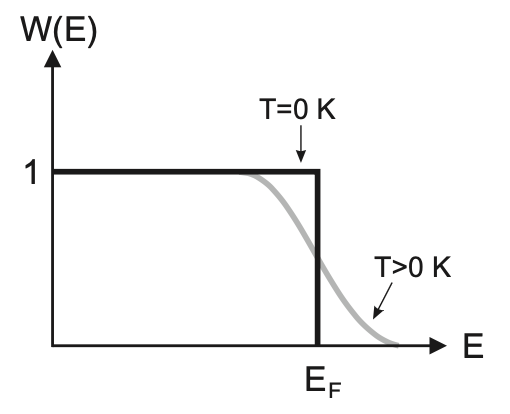
\includegraphics[width=0.6\textwidth]{img/Fermi-energie.png}
    \caption{Energieverteilung der elektronen in einem Metall}\cite{PAPskript}
    \label{fig:energiebandmodell}
\end{figure}

Die Energetischen Zustände können anhand eines Potentialtops in Abbildung \ref{fig:potentialtopf} veranschaulicht werden. Die Leitungselektronen besetzen dort kontinuierliche Zustände bis zur Fermi-Energie. Um das Metall verlassen zu können, muss ein Elektron die Austrittsarbeit $A$ aufbringen. Die Austrittsarbeit ist die Energie, die ein Elektron benötigt, um das Metall zu verlassen. Sie ist materialabhängig und liegt im Bereich von einigen Elektronenvolt.
\begin{figure}[H]
    \centering
    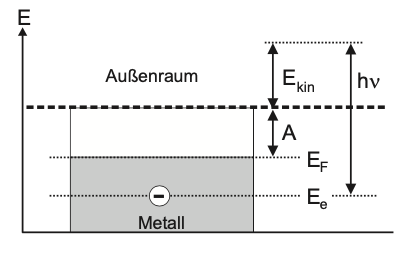
\includegraphics[width=0.6\textwidth]{img/Potentialtopf.png}
    \caption{Potentialtopfmodell eines Metalls}\cite{PAPskript}
    \label{fig:potentialtopf}
\end{figure}

\subsection{Energieverhältnisse beim Fotoeffekt}
Die Energie eines Herausgelösten Elektrons ist die Summe aus der kinetischen Energie $E_{kin}$ und der Austrittsarbeit $A$. 

Die kinetische Energie des Elektrons kann durch die Gegenfeldmethode bestimmt werden. Dabei wird eine Spannung $U$ an die Fotokathode angelegt, die das Elektron aufhält. Die kinetische Energie des Elektrons ist dann gegeben durch:

\begin{equation}
    h\nu = A + (E_F-E_e) + E_{kin}
\end{equation}

Die Maximale kinetische Energie der Elektronen findet an der Fermi-Kante statt. Die kinetische Energie der Elektronen ist dann gegeben durch:

\begin{equation}
    E_{kin,max} = h\nu - A
\end{equation}

Es wird für die Durchführung dieser Messung eine Fotozelle verwendet, die aus einer Fotokathode und einer Anode besteht. Die Fotokathode ist mit einer Spannung $U$ gegenüber der Anode aufgeladen. Die Anode ist dabei so geschaltet, dass sie die Elektronen, die von der Fotokathode emittiert werden, aufnimmt.

\begin{figure}[H]
    \centering
    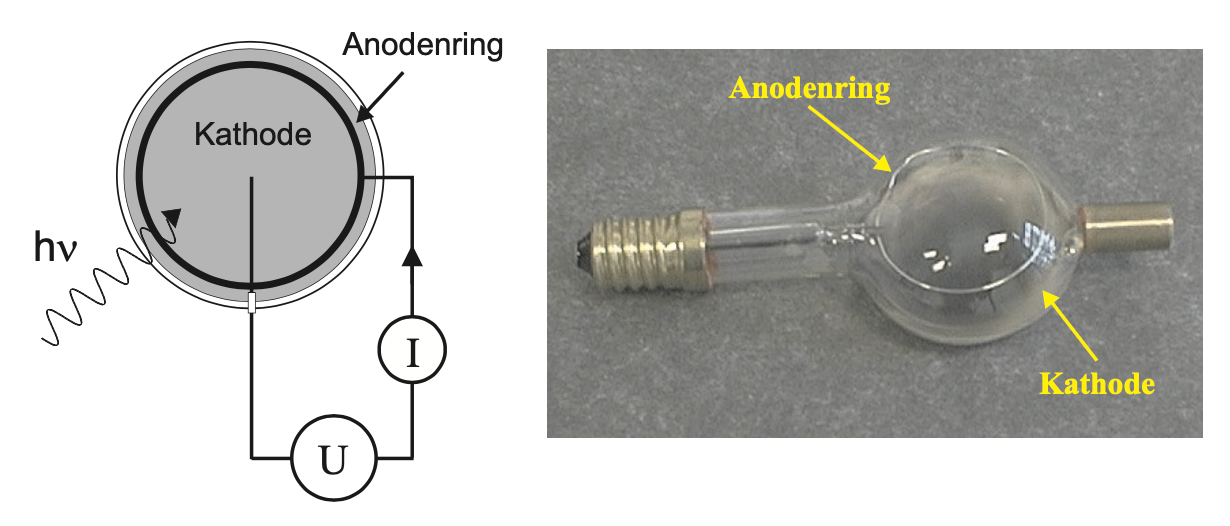
\includegraphics[width=0.6\textwidth]{img/Fotozelle.png}
    \caption{Schematische Darstellung einer Fotozelle}\cite{PAPskript}
    \label{fig:fotozelle}
\end{figure}


Mithilfe einer Gegenfeldmethode kann die maximale kinetische Energie der Elektronen bestimmt werden. Dabei wird eine Spannung $U$ an die Fotokathode angelegt, die die Elektronen mit steigender Spannnung abbremst. Bei einer Sperrspannnung $U_s$ wird der Strom null. Die kinetische Energie des Elektrons ist dann gegeben durch:

\begin{equation}
    E_{kin,max} = eU_s
\end{equation}

Damit wirklich die Fotoelektronen auf die Anode treffen, muss eine hohe positve Saugspannung wirken. Die Saugspannung ist die Spannung, die an der Anode angelegt wird, um die Elektronen aufzufangen. Um $U_s$ bei $T > 0\,\text{K}$ zu bestimmen, muss der funktionale Verlauf der Strom-Spannungs-Kennlinie bekannt sein. Die verwendeete Fotozelle besitzt ungefähr die Funktion:
\begin{equation}
    I \propto U^2
\end{equation}

Bei der Auswertung wird Gerade $\sqrt{I}$ gegen $U$ aufgetragen. Die Schnittstelle mit der Spannung $U$ ist dann die Sperrspannung $U_s$. Die kinetische Energie der Elektronen ist dann gegeben durch:
\begin{equation}
    E_{kin,max} = eU_s = h\nu - A 
\end{equation}

\begin{figure}[H]
    \centering
    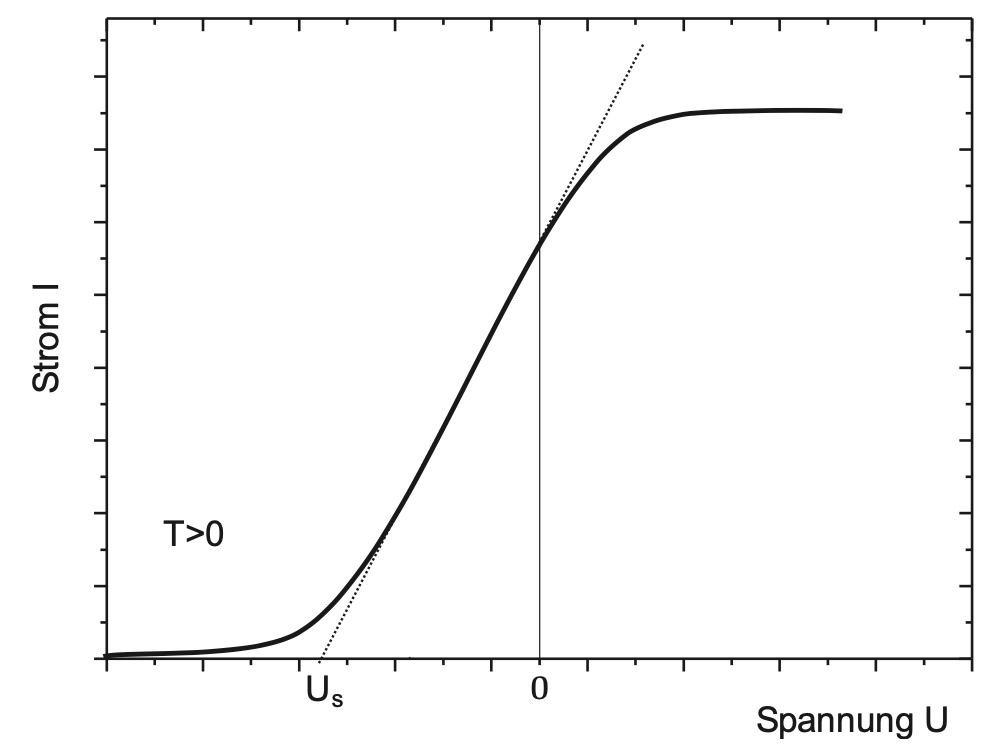
\includegraphics[width=0.6\textwidth]{img/Strom-Spannungs-Kennlinie.png}
    \caption{Strom-Spannungs-Kennlinie}\cite{PAPskript}
    \label{fig:gegenfeldmethode}
\end{figure}


\subsection{Bestimmung des Planckschen Wirkungsquantums}

Um das Plancksche Wirkungsquantum $h$ zu bestimmen, wird die ermittelte Sperrspannung $U_s$ gegen die Frequenz $\nu$ des eingestrahlten Lichts aufgetragen. Die Frequenz des Lichts berechnet sich aus der Wellenlänge $\lambda$ und der Lichtgeschwindigkeit $c$ durch:
\begin{equation}
    \nu = \frac{c}{\lambda}
\end{equation}

Nach der Einsteinschen Gleichung für den Fotoeffekt besteht zwischen der Sperrspannung und der Frequenz der folgende lineare Zusammenhang:
\begin{equation}
    U_s(\nu) = \frac{h}{e} \cdot \nu - \frac{A}{e}
\end{equation}

Beim Auftragen von $U_s$ gegen $\nu$ ergibt sich somit eine Gerade, deren Steigung $m$ dem Verhältnis $\frac{h}{e}$ entspricht. Das Plancksche Wirkungsquantum berechnet sich daher aus der experimentell ermittelten Steigung der Ausgleichsgeraden multipliziert mit der Elementarladung $e$:
\begin{equation}
    h = m \cdot e = \frac{\Delta U_s}{\Delta \nu} \cdot e
\end{equation}

\section{Messprotokoll}
\subsection{Versuchsaufbau und Aufgaben}

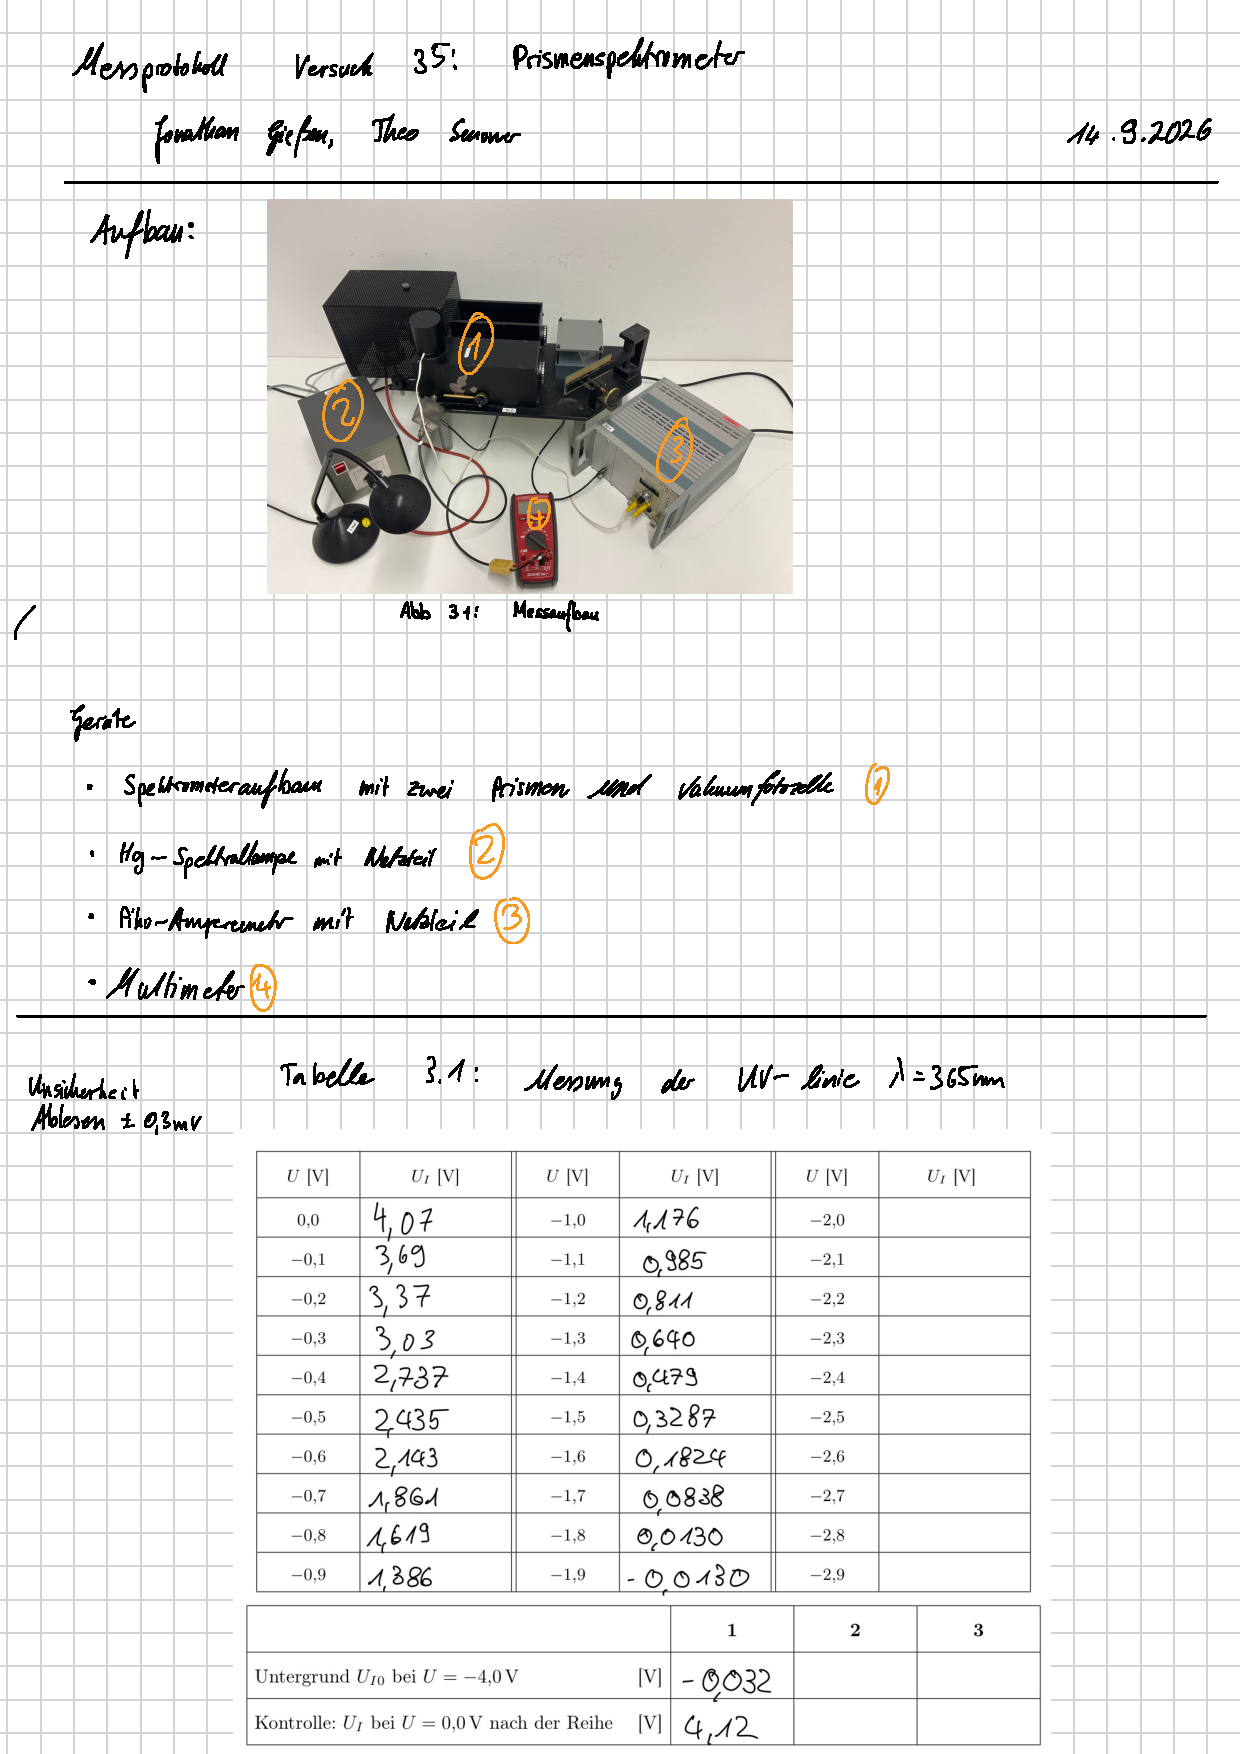
\includepdf[
    pages=-,
    width=\textwidth,
    height=\textheight,
    keepaspectratio,
    pagecommand={\thispagestyle{scrheadings}},
    pagecommand*={\thispagestyle{scrheadings}}
]{../Messprotokoll 35.pdf}


\subsection{Hinweis zum Aufbau}

Der Versuchsaufbau basiert auf einem Spektrometer, das zur Erhöhung der Dispersion zwei hintereinander geschaltete Flintglasprismen nutzt. Über einen beweglichen Spiegel werden die einzelnen Spektrallinien des Lichts gezielt durch einen Austrittsspalt auf die Fotokathode einer Fotozelle gelenkt. Zur visuellen Kontrolle und Ausrichtung kann das Licht mit einem schwenkbaren Spiegel vorübergehend auf einen eingebauten Papierschirm geworfen werden; durch die Fluoreszenz des Papiers wird dort sogar die UV-Linie bei $365,0\,\text{nm}$ sichtbar\cite{PAPskript}. 

Da die beim Fotoeffekt emittierten Elektronen nur extrem kleine Fotoströme im Bereich von einigen $10\,\text{pA}$ erzeugen, müssen diese für die Messung verstärkt werden. Dies geschieht durch einen Strom-Spannungswandler, bei dem der von der Fotozelle gelieferte Strom durch einen Widerstand von $1\,\text{G}\Omega$ fließt, und einen nachgeschalteten hochohmigen Verstärker, der das Signal nochmals um den Faktor 11 verstärkt. Der Fotostrom wird somit indirekt über eine proportionale Spannung $U_I$ gemessen, wobei eine abgelesene Spannung von $1\,\text{V}$ einem tatsächlichen Strom von $91\,\text{pA}$ entspricht\cite{PAPskript}.


\subsection{Durchführung}
Es werden die Spektrallinien der Hg-Spektrallampe nacheinander auf die Fotokathode der Fotozelle gerichtet. Damit die Linie perfekt die Fotokathode erreicht, wird die Spiegelposition durch Maximierung des Photostroms bestimmt. Für jede Spektrallinie wird die Strom-Spannungs-Kennlinie aufgenommen, indem die Spannung $U$ an der Fotokathode variiert und der entsprechende Fotostrom $I$ gemessen wird. Die Messung erfolgt für fünf ausgewählte Spektrallinien im Bereich von $365,0\,\text{nm}$ bis $579,1\,\text{nm}$.

\section{Auswertung}

\subsection{Fehlerrechnung}

Der Fehler des Messgeräts ist vom Messbereich abhängig. Auf dem Datenblatt des Mulitmeters lässt sich ablesen:
\begin{table}[H]
\centering
\caption{Fehler des Multimeters}
\begin{tabular}{|c|c|c|}
    \toprule
    \textbf{Messbereich} & \textbf{Auflösung $\zeta$} & \textbf{Messgenauigkeit $\eta$}\\
    \midrule
    $400\,\text{mV}$ & $100\,\mu\text{V}$ & $\pm(0,25\% + 5\,\text{Digit})$\\
    $4\,\text{V}$ & $1\,\text{mV}$ & $\pm(0,4\% + 1\,\text{Digit})$\\
    $40\,\text{V}$ & $10\,\text{mV}$ & $\pm(0,25\% + 1\,\text{Digit})$\\
    $400\,\text{V}$ & $100\,\text{mV}$ & $\pm(0,25\% + 1\,\text{Digit})$\\
    $1000\,\text{V}$ & $1\,\text{V}$ & $\pm(0,25\% + 1\,\text{Digit})$\\
    \bottomrule
\end{tabular}
\end{table}

Der Fehler des Messgeräts berechnet sich nach der Formel:
\begin{equation}
    \Delta U_{\text{Messgerät}} = \zeta + \eta \cdot U
\end{equation}


Der Gesamtfehler der Messung setzt sich aus dem Ablesefehler und dem Fehler des Messgeräts zusammen. Der Ablesefehler wird auf $0,3,\text{mV}$ geschätzt. Der Gesamtfehler berechnet sich nach der Gaußschen Fehlerfortpflanzung:
\begin{equation}    
    \Delta U = \sqrt{(\Delta U_\text{Ablesen})^2 + (\Delta U_\text{Messgerät})^2}
\end{equation}


\subsection{Berechnungen der Zahlenwerte}\label{sec:Berechnungen der Zahlenwerte}
%% === Tabelle: UV-Linie ($\lambda = 365\,\text{nm}$) ===
\begin{table}[H]
\centering
\caption{Messwerte UV-Linie ($\lambda = 365\,\text{nm}$) (Teil 1)}
\resizebox{\textwidth}{!}{
\begin{tabular}{|c|c|c|c|c|c|c|}
\hline
 $U\,[\text{V}]$ & $0,0$ & $-0,1$ & $-0,2$ & $-0,3$ & $-0,4$ & $-0,5$ \\\hline
 $U_I\,[\text{V}]$ & $4.070 \pm 0.020$ & $3.690 \pm 0.016$ & $3.370 \pm 0.015$ & $3.030 \pm 0.013$ & $2.737 \pm 0.012$ & $2.435 \pm 0.011$ \\\hline
 $U_I - U_{I0}\,[\text{V}]$ & $4.102 \pm 0.020$ & $3.722 \pm 0.016$ & $3.402 \pm 0.015$ & $3.062 \pm 0.013$ & $2.769 \pm 0.012$ & $2.467 \pm 0.011$ \\\hline
 $\sqrt{U_I - U_{I0}}$ & $2.025 \pm 0.005$ & $1.929 \pm 0.004$ & $1.844 \pm 0.004$ & $1.750 \pm 0.004$ & $1.664 \pm 0.004$ & $1.571 \pm 0.004$ \\\hline
\end{tabular}
}
\end{table}

\begin{table}[H]
\centering
\caption{Messwerte UV-Linie ($\lambda = 365\,\text{nm}$) (Teil 2)}
\resizebox{\textwidth}{!}{
\begin{tabular}{|c|c|c|c|c|c|c|}
\hline
 $U\,[\text{V}]$ & $-0,6$ & $-0,7$ & $-0,8$ & $-0,9$ & $-1,0$ & $-1,1$ \\\hline
 $U_I\,[\text{V}]$ & $2.143 \pm 0.010$ & $1.861 \pm 0.009$ & $1.619 \pm 0.008$ & $1.386 \pm 0.007$ & $1.176 \pm 0.006$ & $0.985 \pm 0.005$ \\\hline
 $U_I - U_{I0}\,[\text{V}]$ & $2.175 \pm 0.010$ & $1.893 \pm 0.009$ & $1.651 \pm 0.008$ & $1.418 \pm 0.007$ & $1.208 \pm 0.006$ & $1.017 \pm 0.005$ \\\hline
 $\sqrt{U_I - U_{I0}}$ & $1.475 \pm 0.003$ & $1.376 \pm 0.003$ & $1.285 \pm 0.003$ & $1.191 \pm 0.003$ & $1.099 \pm 0.003$ & $1.008 \pm 0.003$ \\\hline
\end{tabular}
}
\end{table}

\begin{table}[H]
\centering
\caption{Messwerte UV-Linie ($\lambda = 365\,\text{nm}$) (Teil 3)}
\resizebox{\textwidth}{!}{
\begin{tabular}{|c|c|c|c|c|c|c|}
\hline
 $U\,[\text{V}]$ & $-1,2$ & $-1,3$ & $-1,4$ & $-1,5$ & $-1,6$ & $-1,7$ \\\hline
 $U_I\,[\text{V}]$ & $0.811 \pm 0.005$ & $0.640 \pm 0.004$ & $0.479 \pm 0.003$ & $0.329 \pm 0.002$ & $0.182 \pm 0.001$ & $0.084 \pm 0.001$ \\\hline
 $U_I - U_{I0}\,[\text{V}]$ & $0.843 \pm 0.005$ & $0.672 \pm 0.004$ & $0.511 \pm 0.003$ & $0.361 \pm 0.002$ & $0.214 \pm 0.002$ & $0.116 \pm 0.001$ \\\hline
 $\sqrt{U_I - U_{I0}}$ & $0.918 \pm 0.003$ & $0.820 \pm 0.002$ & $0.715 \pm 0.002$ & $0.601 \pm 0.002$ & $0.463 \pm 0.002$ & $0.340 \pm 0.002$ \\\hline
\end{tabular}
}
\end{table}

\begin{table}[H]
\centering
\caption{Messwerte UV-Linie ($\lambda = 365\,\text{nm}$) (Teil 4)}
\begin{tabular}{|c|c|c|}
\hline
 $U\,[\text{V}]$ & $-1,8$ & $-1,9$ \\\hline
 $U_I\,[\text{V}]$ & $0.013 \pm 0.001$ & $-0.013 \pm 0.001$ \\\hline
 $U_I - U_{I0}\,[\text{V}]$ & $0.045 \pm 0.001$ & $0.019 \pm 0.001$ \\\hline
 $\sqrt{U_I - U_{I0}}$ & $0.212 \pm 0.003$ & $0.138 \pm 0.004$ \\\hline
\end{tabular}

\end{table}


% === Tabelle: Violette Linie ($\lambda = 405\,\text{nm}$) ===
\begin{table}[H]
\centering
\caption{Messwerte Violette Linie ($\lambda = 405\,\text{nm}$) (Teil 1)}
\resizebox{\textwidth}{!}{
\begin{tabular}{|c|c|c|c|c|c|c|}
\hline
 $U\,[\text{V}]$ & $0,3$ & $0,2$ & $0,1$ & $0,0$ & $-0,1$ & $-0,2$ \\\hline
 $U_I\,[\text{V}]$ & $4.690 \pm 0.022$ & $4.330 \pm 0.021$ & $3.940 \pm 0.017$ & $3.580 \pm 0.016$ & $3.190 \pm 0.014$ & $2.853 \pm 0.013$ \\\hline
 $U_I - U_{I0}\,[\text{V}]$ & $4.717 \pm 0.022$ & $4.357 \pm 0.021$ & $3.967 \pm 0.017$ & $3.607 \pm 0.016$ & $3.217 \pm 0.014$ & $2.880 \pm 0.013$ \\\hline
 $\sqrt{U_I - U_{I0}}$ & $2.172 \pm 0.005$ & $2.087 \pm 0.005$ & $1.992 \pm 0.004$ & $1.899 \pm 0.004$ & $1.794 \pm 0.004$ & $1.697 \pm 0.004$ \\\hline
\end{tabular}
}
\end{table}

\begin{table}[H]
\centering
\caption{Messwerte Violette Linie ($\lambda = 405\,\text{nm}$) (Teil 2)}
\resizebox{\textwidth}{!}{
\begin{tabular}{|c|c|c|c|c|c|c|}
\hline
 $U\,[\text{V}]$ & $-0,3$ & $-0,4$ & $-0,5$ & $-0,6$ & $-0,7$ & $-0,8$ \\\hline
 $U_I\,[\text{V}]$ & $2.482 \pm 0.011$ & $2.182 \pm 0.010$ & $1.862 \pm 0.009$ & $1.584 \pm 0.008$ & $1.325 \pm 0.007$ & $1.089 \pm 0.006$ \\\hline
 $U_I - U_{I0}\,[\text{V}]$ & $2.509 \pm 0.011$ & $2.209 \pm 0.010$ & $1.889 \pm 0.009$ & $1.611 \pm 0.008$ & $1.352 \pm 0.007$ & $1.116 \pm 0.006$ \\\hline
 $\sqrt{U_I - U_{I0}}$ & $1.584 \pm 0.004$ & $1.486 \pm 0.003$ & $1.374 \pm 0.003$ & $1.269 \pm 0.003$ & $1.163 \pm 0.003$ & $1.056 \pm 0.003$ \\\hline
\end{tabular}
}
\end{table}

\begin{table}[H]
\centering
\caption{Messwerte Violette Linie ($\lambda = 405\,\text{nm}$) (Teil 3)}
\resizebox{\textwidth}{!}{
\begin{tabular}{|c|c|c|c|c|c|c|}
\hline
 $U\,[\text{V}]$ & $-0,9$ & $-1,0$ & $-1,1$ & $-1,2$ & $-1,3$ & $-1,4$ \\\hline
 $U_I\,[\text{V}]$ & $0.872 \pm 0.005$ & $0.686 \pm 0.004$ & $0.501 \pm 0.003$ & $0.322 \pm 0.002$ & $0.165 \pm 0.001$ & $0.066 \pm 0.001$ \\\hline
 $U_I - U_{I0}\,[\text{V}]$ & $0.899 \pm 0.005$ & $0.713 \pm 0.004$ & $0.528 \pm 0.003$ & $0.349 \pm 0.002$ & $0.192 \pm 0.001$ & $0.093 \pm 0.001$ \\\hline
 $\sqrt{U_I - U_{I0}}$ & $0.948 \pm 0.003$ & $0.844 \pm 0.002$ & $0.726 \pm 0.002$ & $0.591 \pm 0.002$ & $0.438 \pm 0.002$ & $0.305 \pm 0.002$ \\\hline
\end{tabular}
}
\end{table}

\begin{table}[H]
\centering
\caption{Messwerte Violette Linie ($\lambda = 405\,\text{nm}$) (Teil 4)}
\begin{tabular}{|c|c|c|}
\hline
 $U\,[\text{V}]$ & $-1,5$ & $-1,6$ \\\hline
 $U_I\,[\text{V}]$ & $0.006 \pm 0.001$ & $-0.014 \pm 0.001$ \\\hline
 $U_I - U_{I0}\,[\text{V}]$ & $0.032 \pm 0.001$ & $0.013 \pm 0.001$ \\\hline
 $\sqrt{U_I - U_{I0}}$ & $0.180 \pm 0.003$ & $0.114 \pm 0.005$ \\\hline
\end{tabular}

\end{table}


% === Tabelle: Blaue Linie ($\lambda = 436\,\text{nm}$) ===
\begin{table}[H]
\centering
\caption{Messwerte Blaue Linie ($\lambda = 436\,\text{nm}$) (Teil 1)}
\resizebox{\textwidth}{!}{
\begin{tabular}{|c|c|c|c|c|c|c|}
\hline
 $U\,[\text{V}]$ & $0,3$ & $0,2$ & $0,1$ & $0,0$ & $-0,1$ & $-0,2$ \\\hline
 $U_I\,[\text{V}]$ & $6.080 \pm 0.026$ & $5.580 \pm 0.024$ & $5.040 \pm 0.023$ & $4.560 \pm 0.022$ & $3.990 \pm 0.017$ & $3.544 \pm 0.015$ \\\hline
 $U_I - U_{I0}\,[\text{V}]$ & $6.119 \pm 0.026$ & $5.619 \pm 0.024$ & $5.079 \pm 0.023$ & $4.599 \pm 0.022$ & $4.029 \pm 0.017$ & $3.583 \pm 0.016$ \\\hline
 $\sqrt{U_I - U_{I0}}$ & $2.474 \pm 0.005$ & $2.371 \pm 0.005$ & $2.254 \pm 0.005$ & $2.145 \pm 0.005$ & $2.007 \pm 0.004$ & $1.893 \pm 0.004$ \\\hline
\end{tabular}
}
\end{table}

\begin{table}[H]
\centering
\caption{Messwerte Blaue Linie ($\lambda = 436\,\text{nm}$) (Teil 2)}
\resizebox{\textwidth}{!}{
\begin{tabular}{|c|c|c|c|c|c|c|}
\hline
 $U\,[\text{V}]$ & $-0,3$ & $-0,4$ & $-0,5$ & $-0,6$ & $-0,7$ & $-0,8$ \\\hline
 $U_I\,[\text{V}]$ & $3.097 \pm 0.014$ & $2.654 \pm 0.012$ & $2.252 \pm 0.010$ & $1.840 \pm 0.009$ & $1.479 \pm 0.007$ & $1.175 \pm 0.006$ \\\hline
 $U_I - U_{I0}\,[\text{V}]$ & $3.136 \pm 0.014$ & $2.693 \pm 0.012$ & $2.291 \pm 0.010$ & $1.879 \pm 0.009$ & $1.518 \pm 0.007$ & $1.214 \pm 0.006$ \\\hline
 $\sqrt{U_I - U_{I0}}$ & $1.771 \pm 0.004$ & $1.641 \pm 0.004$ & $1.514 \pm 0.003$ & $1.371 \pm 0.003$ & $1.232 \pm 0.003$ & $1.102 \pm 0.003$ \\\hline
\end{tabular}
}
\end{table}

\begin{table}[H]
\centering
\caption{Messwerte Blaue Linie ($\lambda = 436\,\text{nm}$) (Teil 3)}
\resizebox{\textwidth}{!}{
\begin{tabular}{|c|c|c|c|c|c|c|}
\hline
 $U\,[\text{V}]$ & $-0,9$ & $-1,0$ & $-1,1$ & $-1,2$ & $-1,3$ & $-1,4$ \\\hline
 $U_I\,[\text{V}]$ & $0.870 \pm 0.005$ & $0.577 \pm 0.004$ & $0.310 \pm 0.002$ & $0.119 \pm 0.001$ & $0.013 \pm 0.001$ & $-0.021 \pm 0.001$ \\\hline
 $U_I - U_{I0}\,[\text{V}]$ & $0.909 \pm 0.005$ & $0.616 \pm 0.004$ & $0.350 \pm 0.002$ & $0.158 \pm 0.001$ & $0.052 \pm 0.001$ & $0.019 \pm 0.001$ \\\hline
 $\sqrt{U_I - U_{I0}}$ & $0.954 \pm 0.003$ & $0.785 \pm 0.002$ & $0.591 \pm 0.002$ & $0.398 \pm 0.002$ & $0.228 \pm 0.003$ & $0.136 \pm 0.005$ \\\hline
\end{tabular}
}
\end{table}


% === Tabelle: Grüne Linie ($\lambda = 546\,\text{nm}$) ===
\begin{table}[H]
\centering
\caption{Messwerte Grüne Linie ($\lambda = 546\,\text{nm}$) (Teil 1)}
\resizebox{\textwidth}{!}{
\begin{tabular}{|c|c|c|c|c|c|c|}
\hline
 $U\,[\text{V}]$ & $0,3$ & $0,2$ & $0,1$ & $0,0$ & $-0,1$ & $-0,2$ \\\hline
 $U_I\,[\text{V}]$ & $3.049 \pm 0.013$ & $2.530 \pm 0.011$ & $2.033 \pm 0.009$ & $1.547 \pm 0.007$ & $1.132 \pm 0.006$ & $0.776 \pm 0.004$ \\\hline
 $U_I - U_{I0}\,[\text{V}]$ & $3.065 \pm 0.014$ & $2.546 \pm 0.011$ & $2.049 \pm 0.009$ & $1.563 \pm 0.008$ & $1.148 \pm 0.006$ & $0.792 \pm 0.004$ \\\hline
 $\sqrt{U_I - U_{I0}}$ & $1.751 \pm 0.004$ & $1.596 \pm 0.004$ & $1.432 \pm 0.003$ & $1.250 \pm 0.003$ & $1.072 \pm 0.003$ & $0.890 \pm 0.003$ \\\hline
\end{tabular}
}
\end{table}

\begin{table}[H]
\centering
\caption{Messwerte Grüne Linie ($\lambda = 546\,\text{nm}$) (Teil 2)}
\begin{tabular}{|c|c|c|c|c|}
\hline
 $U\,[\text{V}]$ & $-0,3$ & $-0,4$ & $-0,5$ & $-0,6$ \\\hline
 $U_I\,[\text{V}]$ & $0.477 \pm 0.003$ & $0.266 \pm 0.001$ & $0.120 \pm 0.001$ & $0.047 \pm 0.001$ \\\hline
 $U_I - U_{I0}\,[\text{V}]$ & $0.493 \pm 0.003$ & $0.282 \pm 0.002$ & $0.136 \pm 0.001$ & $0.064 \pm 0.001$ \\\hline
 $\sqrt{U_I - U_{I0}}$ & $0.702 \pm 0.002$ & $0.531 \pm 0.002$ & $0.369 \pm 0.002$ & $0.252 \pm 0.002$ \\\hline
\end{tabular}

\end{table}


% === Tabelle: Gelbe Linie ($\lambda = 578\,\text{nm}$) ===
\begin{table}[H]
\centering
\caption{Messwerte Gelbe Linie ($\lambda = 578\,\text{nm}$) (Teil 1)}
\resizebox{\textwidth}{!}{
\begin{tabular}{|c|c|c|c|c|c|c|}
\hline
 $U\,[\text{V}]$ & $0,3$ & $0,2$ & $0,1$ & $0,0$ & $-0,1$ & $-0,2$ \\\hline
 $U_I\,[\text{V}]$ & $0.584 \pm 0.004$ & $0.405 \pm 0.003$ & $0.262 \pm 0.001$ & $0.164 \pm 0.001$ & $0.099 \pm 0.001$ & $0.066 \pm 0.001$ \\\hline
 $U_I - U_{I0}\,[\text{V}]$ & $0.591 \pm 0.004$ & $0.412 \pm 0.003$ & $0.269 \pm 0.002$ & $0.171 \pm 0.001$ & $0.106 \pm 0.001$ & $0.073 \pm 0.001$ \\\hline
 $\sqrt{U_I - U_{I0}}$ & $0.769 \pm 0.002$ & $0.642 \pm 0.002$ & $0.519 \pm 0.002$ & $0.414 \pm 0.002$ & $0.325 \pm 0.002$ & $0.270 \pm 0.002$ \\\hline
\end{tabular}
}
\end{table}

\begin{table}[H]
\centering
\caption{Messwerte Gelbe Linie ($\lambda = 578\,\text{nm}$) (Teil 2)}
\begin{tabular}{|c|c|c|c|c|}
\hline
 $U\,[\text{V}]$ & $-0,3$ & $-0,4$ & $-0,5$ & $-0,6$ \\\hline
 $U_I\,[\text{V}]$ & $0.048 \pm 0.001$ & $0.035 \pm 0.001$ & $0.028 \pm 0.001$ & $0.022 \pm 0.001$ \\\hline
 $U_I - U_{I0}\,[\text{V}]$ & $0.054 \pm 0.001$ & $0.042 \pm 0.001$ & $0.035 \pm 0.001$ & $0.029 \pm 0.001$ \\\hline
 $\sqrt{U_I - U_{I0}}$ & $0.233 \pm 0.003$ & $0.205 \pm 0.003$ & $0.187 \pm 0.003$ & $0.169 \pm 0.003$ \\\hline
\end{tabular}
\end{table}












\clearpage

\listoffigures


\listoftables

\begin{thebibliography}{5}
    \bibitem{PAPskript} Dr. J.Wagner, \emph{Physikalisches Anfängerpraktikum}, Stand 11/2024
    \bibitem{ilberg1988physikalisches} W. Ilberg, M. Krötzsch, \emph{Physikalisches Praktikum für Anfänger}, BSB B. G. Teubner Verlagsgesellschaft, Leipzig (1985).
\end{thebibliography}




\begin{comment}

\begin{table}[H]
    \centering
    \caption{Mess- und Geräteparameter für die exemplarische Berechnung (Messung 28).}
    \label{tab:parameter_messung_28}
    \begin{tabular}{ll}
        \toprule
        \textbf{Größe} & \textbf{Wert} \\
        \midrule
        Fallstrecke & $s_1 = 10\,\text{Skt} = 5.00 \cdot 10^{-4}\,\text{m}$ \\
        Fallzeit & $t_1 = 11.85\,\text{s}$ \\
        Steigstrecke & $s_2 = 10\,\text{Skt} = 5.00 \cdot 10^{-4}\,\text{m}$ \\
        Steigzeit & $t_2 = 18.19\,\text{s}$ \\
        Skalenteilung & $1\,\text{Skt} = 5.00 \cdot 10^{-5}\,\text{m}$ \\
        Kondensatorspannung & $U = 500\,\text{V}$ \\
        Plattenabstand & $d = 6.00 \cdot 10^{-3}\,\text{m}$ \\
        Luftdruck & $p = 100285\,\text{Pa}$ \\
        Erdbeschleunigung & $g = 9.81\,\frac{\text{m}}{\text{s}^2}$ \\
        Dichtedifferenz & $\rho = \rho_{\text{Öl}} - \rho_{\text{Luft}} = 871.21\,\frac{\text{kg}}{\text{m}^3}$ \\
        Unkorrigierte Luftviskosität & $\eta_0 = 1.81 \cdot 10^{-5}\,\text{Pa}\cdot\text{s}$ \\
        Cunningham-Konstante & $b = 7.78 \cdot 10^{-3}\,\text{Pa}\cdot\text{m}$ \\
        \bottomrule
    \end{tabular}
\end{table}
\end{comment}
\end{document}